
	In this chapter the concept for the interface design is described, as the design itself and the options taken for the design of the interaction systems.

\section{Concept}

	To achieve our goal of comparing several interaction devices we used several interface systems, a typical \ac{GUI} interface on a computer, a typical \ac{DPad} control interface, a motor control interface with the \ac{Wiimote}, a kinematic control interface also with the \ac{Wiimote}, a kinematic control interface with the Kinect sensor, and a motor control interface with the Kinect sensor. The interaction methods developed were created to control the iCub robot movement, particularly to do arm tasks, such as touching objects or following paths. Trying to achieve precision, natural movement characteristics and intuitive interaction for the iCub movements was a important goal. Although the precision intended was difficult to achieve, due to the iCub limitations, provide interaction methods and experiments that illustrate the advantages and disadvantages of each of the interfaces and their use.
	
	The devices used for this study were a computer \ac{GUI}, a \acf{Wiimote}, and a Kinect sensor. The computer \ac{GUI} had already been developed, and it is broadly used and accepted by the iCub development community as the default interface for the iCub motor control. The \ac{Wiimote} interfaces and Kinect interfaces are novel contributions of this work.

\section{iCub}

	The iCub robot is a humanoid robot with 53 \ac{DOF}. To control each motor it is first needed to declare a part of the robot (head, torso, legs, or arms), where the motor is located, this is part of a three level tree, where the levels correspond to: robot, part, and motor. Within each part the motors are identified by sequential numbers, that start from 0 to the value of \ac{DOF} of the part accessed.

	The software used to control the iCub can be downloaded from the iCub \ac{SVN}\footnote{\url{https://robotcub.svn.sourceforge.net/svnroot/robotcub/trunk/iCub}}, although there is a binary version available it is preferred to compile the source available with the latest updates.
	
	The iCub software was developed as open source software, so it is a result of a series of contributions to the iCub project done by different individuals from different places. This makes the iCub repository very broad in its goals, just as there are applications to control the robot motors, there are also image processing applications, or robot learning applications. Many of this applications are divided into modules that can be reused with modules other than the original ones. 
	
	A example of a module is the iKin Solver that uses the iKin Controller, and that is able to receive a 3D Cartesian point (where the root point is between the legs of the robot), and use the inverse kinematics of the iCub robot to make the robot end-effector move to the specified point. The end-effector in the arm case is typically the hand of the robot, but another end-effector can be specified, such as the shoulder, elbow, or any of the robots joints. Any program developed can use these modules that were implemented exactly to be used as support utilities for other programs.
	
	The \ac{GUI} used can be found in the iCub repository, but the \ac{Wiimote} and Kinect interaction modules were designed following the approach used by modules already available and are ready to be used for other purposes than solely the control of the iCub arm, both of the modules also take advantage of some software available in the iCub repository, such as the iKin driver, or the motor control devices.

\section{\acf{GUI}}

	The \ac{GUI} used to ``control'' the iCub motors is a part of the iCub software repository, so no development was needed.
	
	\begin{figure}[htb]
	\begin{center}
	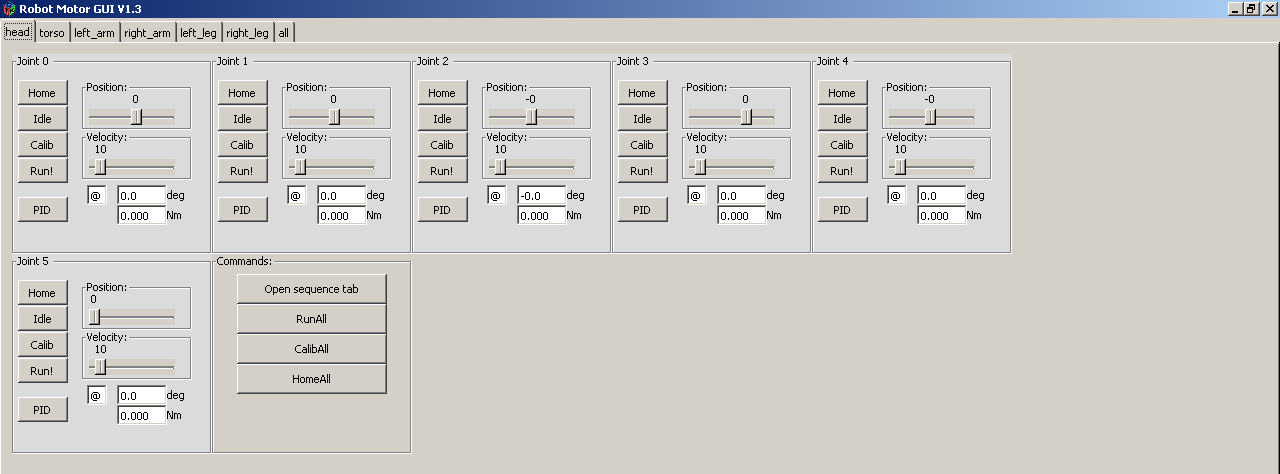
\includegraphics[width=150mm]{robotMotorGui.png}
	\end{center}
	\caption[Computer motor interface]{Computer motor interface - named robotMotorGui.} 
	\label{fig:robotMotorGui}
	\end{figure}
	
	A screenshot of the the \ac{GUI} used is shown on figure \ref{fig:robotMotorGui}. The \ac{GUI} divides each of the iCub parts into tabs, and a ``all'' tab that joins all the controls presented in each tab into a single one. Each tab is subdivided into a set of control panels equal the number of motors in that part, or in case of the kinematic control tabs there are three panels to control the Cartesian position of the end-effector and three panels to control the orientation of the end-effector, both tabs have one more panel with buttons that do predefined actions, such as moving the motors to predefined angles, or to move the motors through a user defined sequence of angles.
	
	The control panels can either control the motors of the iCub independently or control a specific iCub end-effector, such as a hand, each panel contains a set of buttons and sliders that move the motor to a predefined angle, or that run a sequence of user defined angles, the same happens with the kinematic control where each panel controls a Cartesian value or a Euler angle, for position or orientation of the end-effector. Also in the panel there are a couple of integer labels that work as output of the motor position and current velocity, or the end-effector Cartesian position and orientation angle. By moving the angle or velocity slider the user can move and alter the motor status, the same happens for the kinematic control. When controlling the kinematics of the robot through a panel, each time that a slider is altered making the robot move to a new pose, the user must wait for the robot to reach its target or for the time specified to reach a target to end, so that the slider can be changed again. When a target position is not reached a warning message is displayed.
	
	The \ac{GUI} is a complex interface made out of simple parts, it becomes complex mainly because of the amount of controls that are available to the user, and also because while controlling the motors, repositioning one motor will affect the position of other motors, obliging the task of repositioning the robot into a specific position, to be done in one previously planned sequence. To be agile in this logical thought of motor sequence it is important to have a clear idea of how each motor moves, and how the change in position of a  motor will affect the others, this perception is only reached with some practice, although in the kinematic control this idea is simplified because only a target point needs to be set for the whole robot to move towards it.
	
	This system allows for a simple control of the motors, and kinematic chain, subdividing the problem of the motor control into simple independent problems for each motor, and abstracting the kinematic control to a 3D Cartesian position. Although this is a complex interface, it is composed of simple parts, which makes it a comprehensible system.

\section{Wiimote}

	The \ac{Wiimote} interaction software for the iCub was developed specifically for this study.

	The  \ac{Wiimote} is a remote control used for interaction with the Wii gaming console, that equipped with the \acf{MP} extension is able to detect angular motion in three axes, pitch, yaw, and roll, as it is shown in figure \ref{fig:wiimoteAxis}. The \ac{MP} extension adds a gyroscope to the already available sensors list. The sensors available in the \ac{Wiimote} have an world axis that is defined in this way: the Y axis, as being along the \ac{Wiimote}; the Z axis, as the direction perpendicular to the buttons surface on the top of the \ac{Wiimote}; the X axis, has the direction perpendicular the \ac{Wiimote} side.
	
	\begin{figure}[htb]
	\begin{center}
	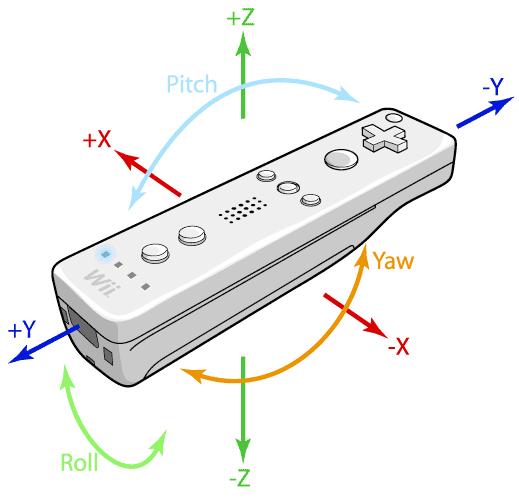
\includegraphics[scale=0.30]{wiimoteAxis.png}
	\end{center}
	\caption[Wii remote axes]{Wii remote axes.} 
	\label{fig:wiimoteAxis}
	\end{figure}
	
	The main difference to other works made on humanoids with the \ac{Wiimote} was using the \ac{MP} extension gyro instead of the \ac{Wiimote} accelerometer, this allows for the detection of a angular movement made with \ac{Wiimote} instead of the \ac{Wiimote} position relatively to gravity. Because it was preferred to track the data from the gyroscope instead of the accelerometer, only the change in angular movements made with the remote are detected.
	
	The buttons on the \ac{Wiimote} were also used, the 1 and 2 button were used, on the motor control, to alter the part being controlled to arm or forearm, in the kinematic control, to alter between controlling the position or controlling the orientation, and the trigger like button B was used to start or stop the control of the robot, while pressed the robot would be controlled, when released the robot stops and clears all the previous commands that were waiting to be executed.
	
	During the work it was avoided to use the \ac{IR} camera because this obliged the users to be always aware that they should be pointing the device to the sensor bar (the \ac{IR} source), and this would not be useful, particularly for the mobile robots.
	
	Although the \ac{Wiimote} control methods presented below can be used to control any part of the robot, they were developed focusing on the robot right arm control, which is the focused part during the evaluation made.

\subsection{Motor control}

	The \ac{Wiimote} motor control, uses the \ac{Wiimote} to interface with each motor independently. A rotation along each of the \ac{Wiimote} axis, controls a different motor. The robot is controlled while the user is pressing the B button, and the motors only move while the user is moving the \ac{Wiimote} with some angular speed.
		
	The arm control is divided into two parts, the arm (motors 0, 1 and 2), and the forearm/hand (motors 3, 4 and 6) parts. The parts angular movements are shown in figure \ref{fig:icubWiimoteMotor} in different colors, and the motors used are shown in figure \ref{fig:icubArm}. The user can toggle between parts using buttons 1 and 2 of the remote. The arm part has three motors that control the three \ac{DOF}, the \ac{Wiimote} are mapped the following way: the Y axis rotation rotates the arm around itself (motor 2, axis 3), the X axis rotation rotates the arm around a axis perpendicular to the robots torso side (motor 0, axis 1), the Z rotation depends on the motor position that is dependent on the X axis rotation (motor 1, axis 2). The forearm part is mapped as: Y axis rotation rotates the forearm around itself (motor 4, axis 5), the X axis rotation rotates the arm around a axis perpendicular to the robots arm (motor 3, axis 4), and the Z rotation rotates the hand left and right in a wave movement (motor 6).
	
	
	\begin{figure}[htb]
	\begin{center}
	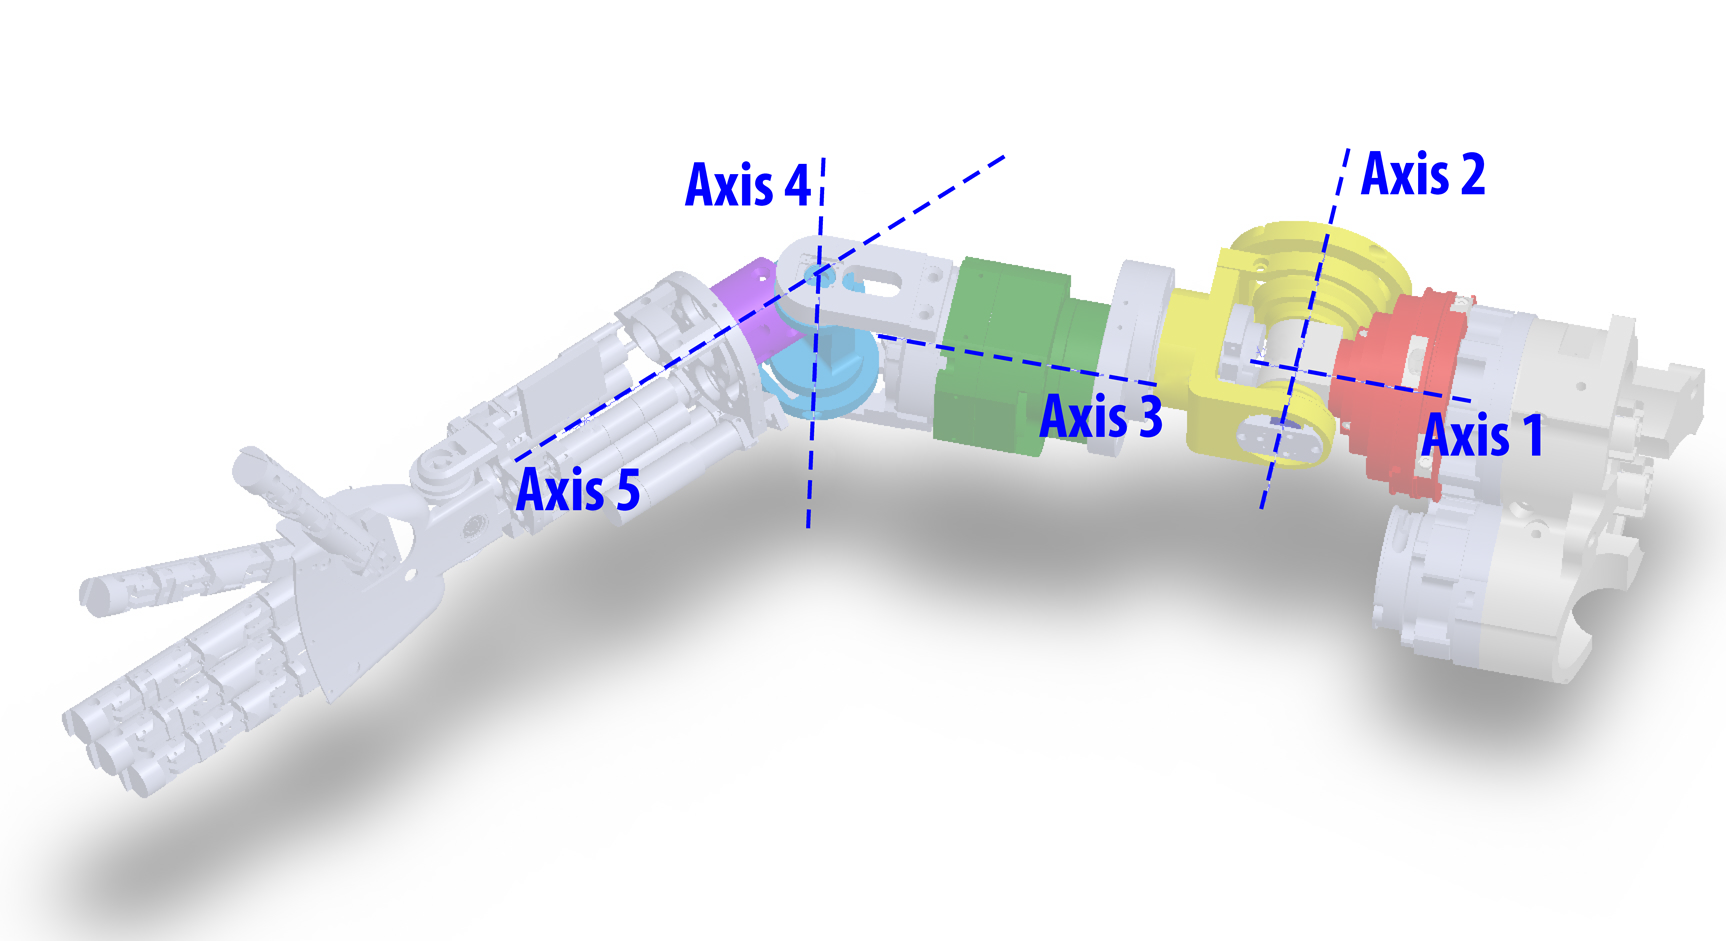
\includegraphics[width=150mm]{icubArm.png}
	\end{center}
	\caption[\ac{Wiimote} controlled motors in the iCub arm]{\ac{Wiimote} controlled motors in the iCub arm.} 
	\label{fig:icubArm}
	\end{figure}
	
	\begin{figure}[htb]
	\begin{center}
	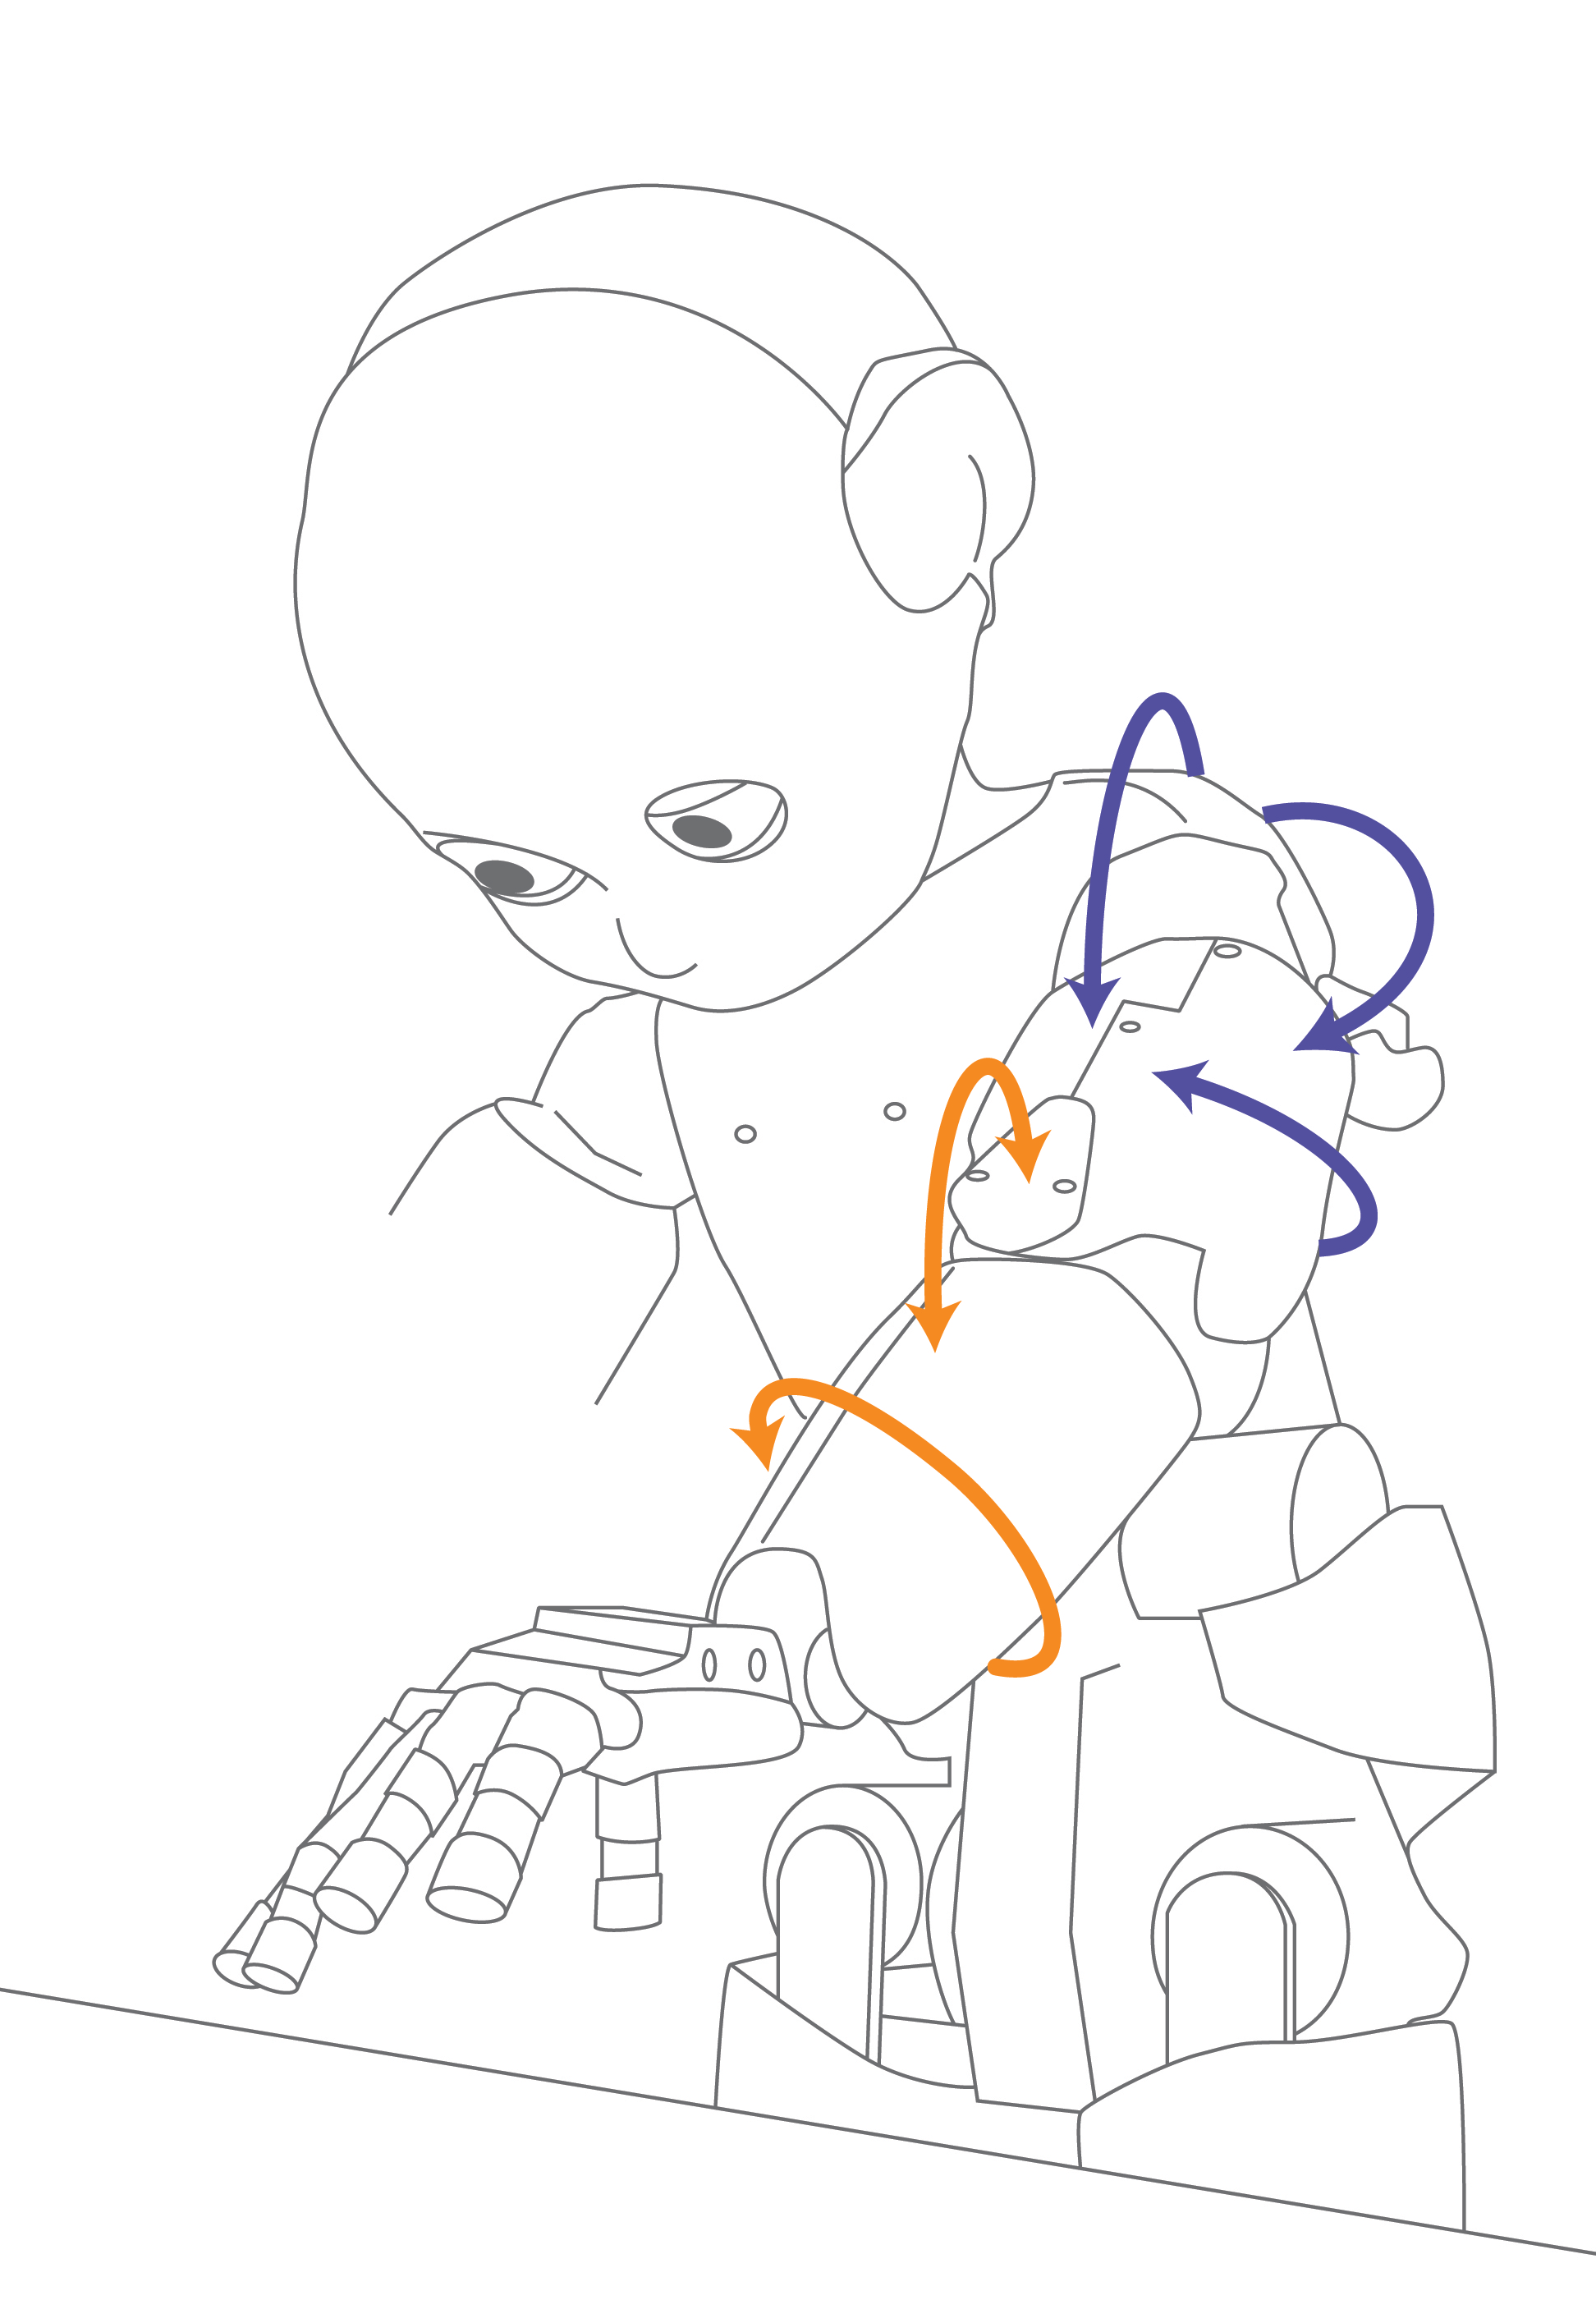
\includegraphics[width=50mm]{icubWiimoteMotor.png}
	\end{center}
	\caption[\ac{Wiimote} motor control of the iCub]{\ac{Wiimote} motor control of the iCub.} 
	\label{fig:icubWiimoteMotor}
	\end{figure}
	
	The control of each motor independently obliges, as the the \ac{GUI} control does, to be aware of the sequence needed to be followed to reach a specific position. The advantage is that this sequence is made out of only two independent parts, that makeup the arm. Each of those part is made up of a maximum of three motors, and the motors are controlled simultaneously by the \ac{Wiimote} angular movements.
	
	There is no need for the user to comprehend how the motors are really positioned because the movements done with the \ac{Wiimote} are mapped to the robots motors. Although the user needs to be aware that this movement mapping does not mean that a movement done by the \ac{Wiimote} will be the movement done by the robot, but that a movement around an axis means a relative movement on a specific motor of the robot.
	
	This system allows a dynamic control of the robot where the motor angles values are abstracted to the user, although the motor rotations and the positions between them are not. This facilitates the control of a single joint, that is composed by multiple motors, of the robot, making it easier to achieve a position through a ``try and fail'' method.

\subsection{Kinematic control}
%solver and d-pad

	The \ac{Wiimote} kinematic control can be used with three different control methods, the \ac{Wiimote} movements can be captured and mapped to the robot, the robot end effector can be positioned using the arrow buttons from the \ac{Wiimote}, or the orientation can be changed through the \ac{Wiimote} movements. The control using the arrow buttons could easily be exported to a computer keyboard or any other device that has six buttons, so it is considered a typical device.
	
	The kinematic control means that the control can be done in relation to an inverse kinematic chain, the user only needs to specify where in the Cartesian space the end-effector should reach, and the robot tries to reach that point. In the \ac{Wiimote} kinematic control method case it means that the angular movements rotate the end-effector around the shoulder of the iCub, having as radius the yellow line and as end-effector the brown ball in the figure \ref{fig:icubWiimoteKinematic}, the cursor control method pressing a button moves the end-effector in a straight way, and the orientation control method does not alter the position of the end-effector only its orientation.
	
	\begin{figure}[htb]
	\begin{center}
	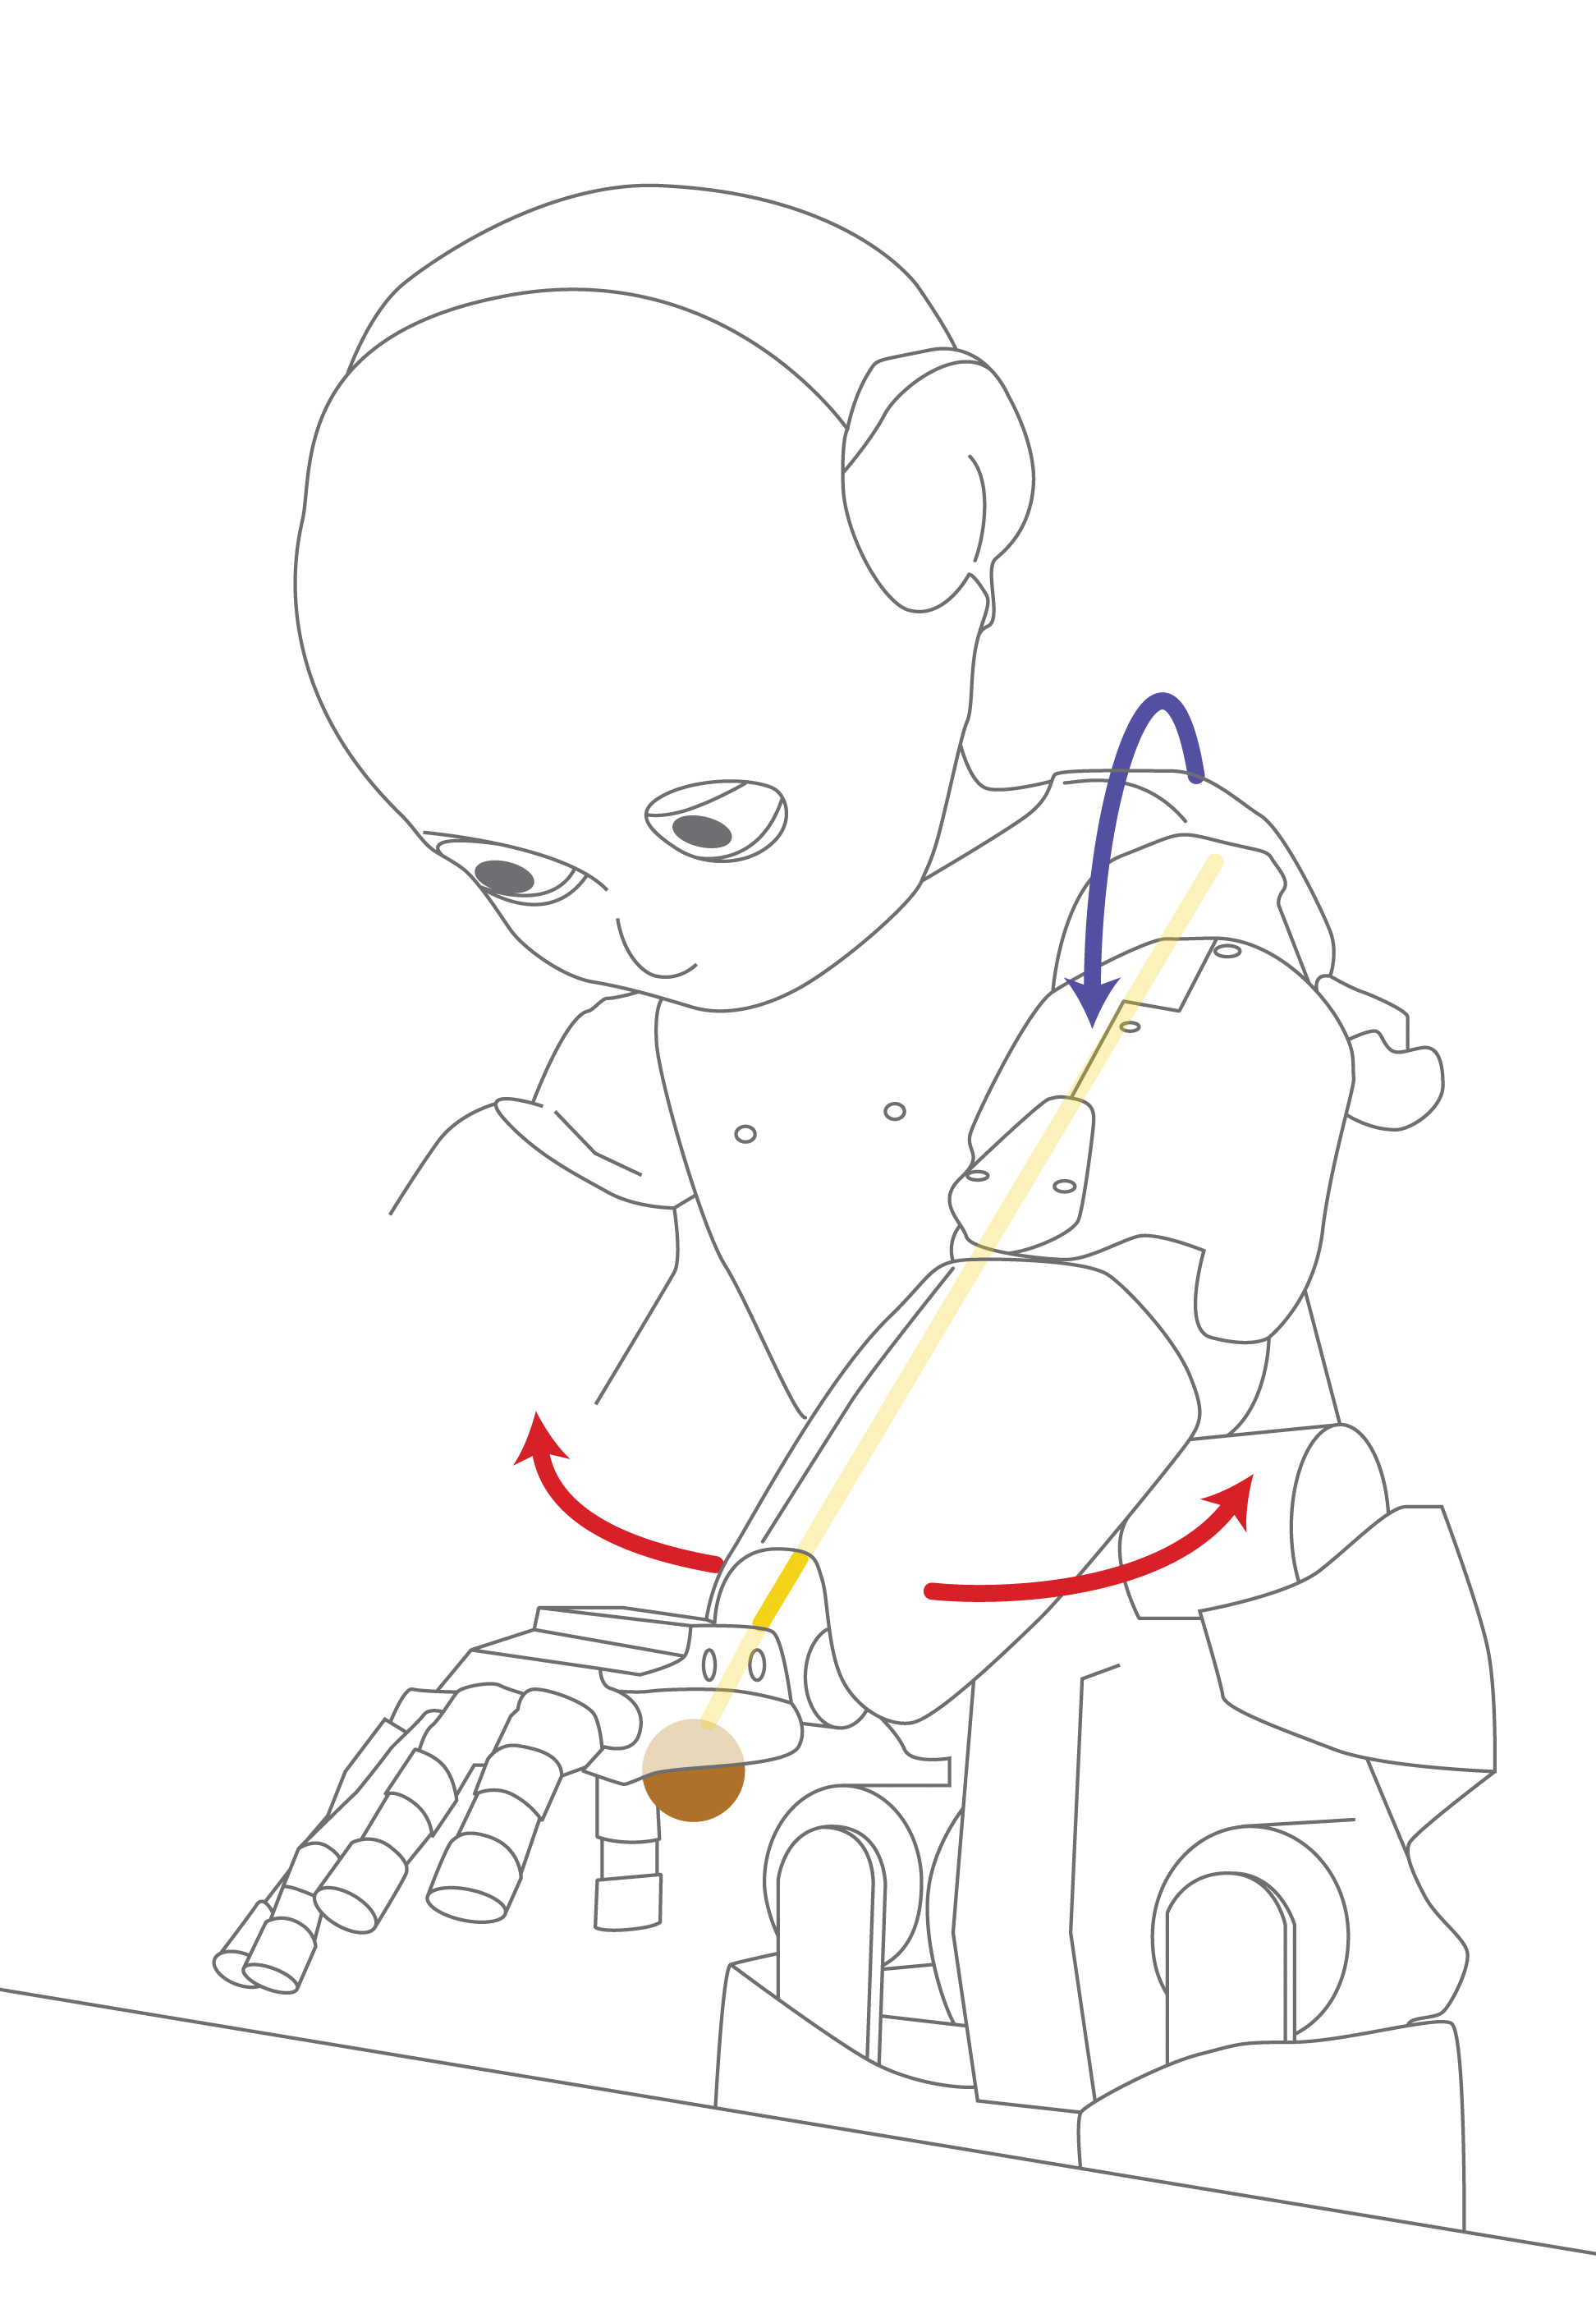
\includegraphics[width=50mm]{icubWiimoteKinematic.png}
	\end{center}
	\caption[\ac{Wiimote} kinematic control of the iCub]{\ac{Wiimote} kinematic control of the iCub.} 
	\label{fig:icubWiimoteKinematic}
	\end{figure}	
	
	In the cursor control method, the end-effector is moved in the space with the cursor and the + and - buttons. The front and back button, move the end-effector to the front of the robot, or to the back of the robot, the left and right buttons, move the end-effector to the left or the right of the robot, the + and - buttons move the end-effector up or down.
	
	In the \ac{Wiimote} kinematic control method, the end effector is moved in space by the movements made with the remote and the + and - buttons, the user only controls the robot while the B button is pressed. The movements of the \ac{Wiimote} are directly mapped into the end-effector position, although because only angular movements can be detected, the end-effector always maintains the same distance from the robots shoulder, this distance can be changed by the + button, that increases the distance, and the - button, that decreases the distance to the shoulder. In other words the angular movements made with the \ac{Wiimote} are mapped in a spherical way to the end-effector, the radius of this sphere can be changed with the + and - buttons, and its center remains in the robot shoulder. In figure \ref{fig:icubWiimoteCursor} this interaction movements is illustrated by arrows.
	
	\begin{figure}[htb]
	\begin{center}
	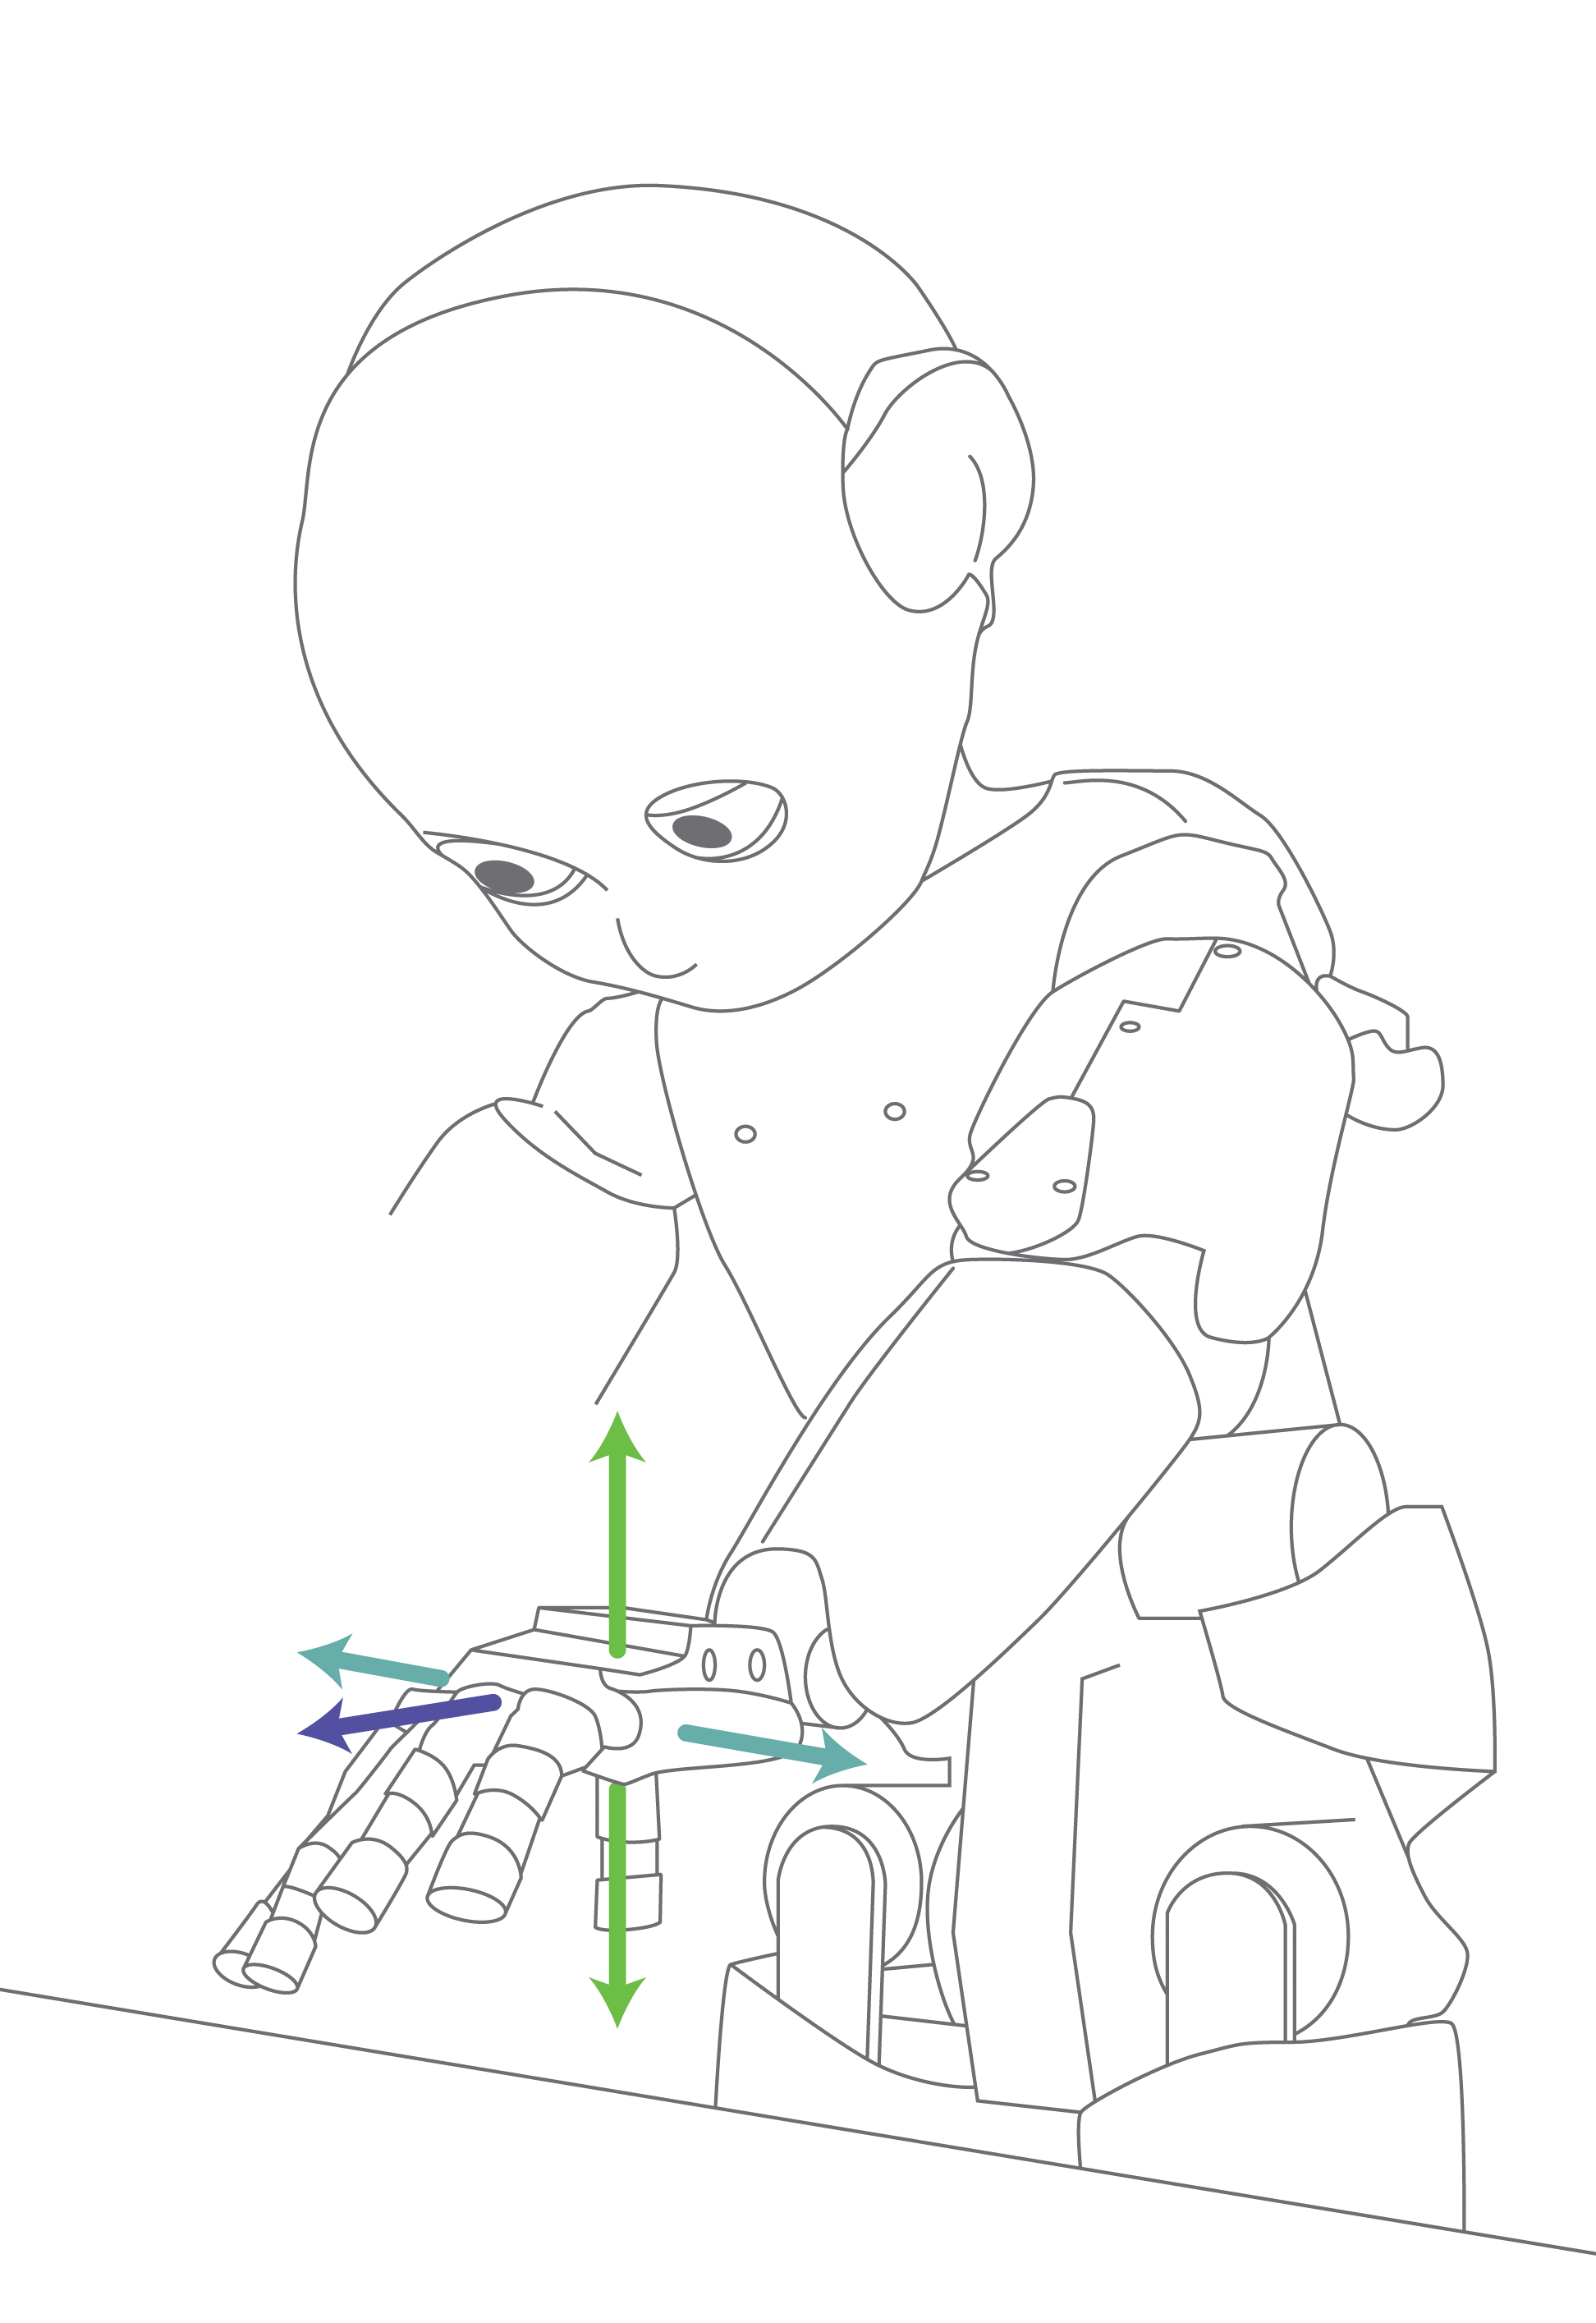
\includegraphics[width=50mm]{icubWiimoteCursor.png}
	\end{center}
	\caption[\ac{Wiimote} cursor control of the iCub]{\ac{Wiimote} cursor control of the iCub.} 
	\label{fig:icubWiimoteCursor}
	\end{figure}	
	
	In the \ac{Wiimote} kinematic orientation control method, the end-effector can be oriented by making angular movements with the remote, as with the \ac{Wiimote} kinematic control method, the control is only made while the B button is pressed. This orientation control method has effect on the end effector orientation, to achieve some orientations of the end-effector the arm must change its configuration, but the Cartesian position of the end-effector is always maintained. Orientation change corresponds to the movement of the \ac{Wiimote}, when a orientation can not be reached, the robot ignores the orientation change request.
	
	This interaction system abstracts the user from any understanding of the motors, their position or angles. The mapping is done directly between the user movements or direction input to the robots end-effector, this is what defines how the motors should be configured to achieve the desired end-effector position. Because the end-effector is a virtual point, there is no way of a user, after having done a movement, having a precise idea of where the end-effector was positioned, so the control is made based on the direction where the user wants the robot to move, and not on the position that the user wants the robot to reach, obliging the user to relay on intuition.

\section{Kinect}

	The Kinect interaction software for the iCub was developed specifically for this study.
	
	The Kinect is a novel remote control for the Xbox 360 gaming console. This device is composed of one RGB, one \ac{IR} camera, an \ac{IR} light source, a microphone, an accelerometer, and a small motor in its base. In this work, only the \ac{IR} camera and the \ac{IR} light source were used.
	
	The Kinect interaction device allows players to interact with the games by moving the body in front of the camera. Typically the movements of the users body are mapped into a avatar character in a game, this work did not stay far from this, but the mapping was done between the user and the iCub, that presents very different challenges than a computer avatar.
		
	\begin{figure}[htb]
	\centering
	  \subfloat[Kinect hand detection.]{\label{fig:kinectHandDetection}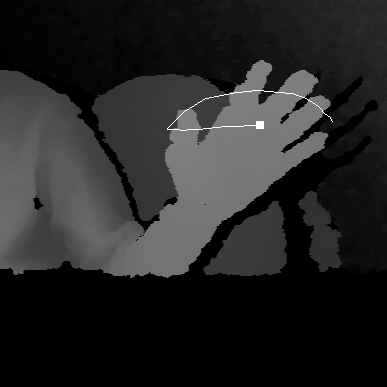
\includegraphics[width=50mm]{CaptureKinectHandSquare.png}}
  \hspace{5mm}
	  \subfloat[Kinect skeleton detection ($\Psi$ calibration pose).] {\label{fig:kinectSkeletonDetection}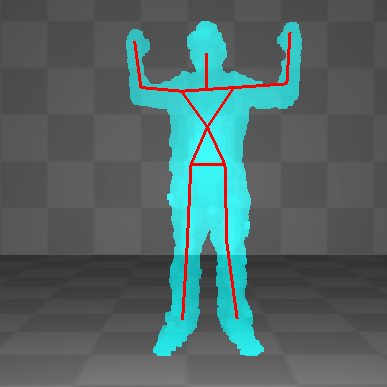
\includegraphics[width=50mm]{CaptureKinectSkeletonPoseSquare.png}}
	\caption{Kinect detection made by sample programs.} 
	\label{fig:kinectDetection}
	\end{figure}
	
	
	A user can be detected by the Kinect device by doing a clear gesture, just by standing in front of the \ac{IR} camera the user pixels in the camera are detected. By waving four times the hand of the user can be detected, and if the user stands in the $\Psi$ position, figure \ref{fig:kinectSkeletonDetection},  with the arms parallel with the floor and the forearms up forming a 90 degrees angle, the skeleton can be detected. These detections are not immediate, they require some seconds and that the user or the hand is fully viewed by the camera, without being too close or too far away.
	
	When a user skeleton is detected by the Kinect, it outputs the user joints in a set of rotation matrices and an 3D Cartesian distance points. The skeleton is made of 24 points and 10 rotation matrices, each of these elements has a confidence value that is between 0 and 1 that indicates how accurate the element might be. If the camera is moved from its original position, the skeleton needs to be recalibrated, which means doing the detection process again.
	
	When the hand is detected it outputs the Cartesian point that is considered to be the center of mass of the hand. This point is continuously followed even if the camera is moved from its original position.
	
	The rotation matrices, and the Cartesian points outputted have their axes and origin defined by the Kinect device position. The Cartesian points can be outputted in centimeters, which are useful for real world coordinate systems, or in pixel values, which are useful for graphical interfaces.
	
	To start and stop the Kinect control, it was decided to use the \ac{Wiimote}, trigger like B button. This allowed to start and stop the control with a subtle movement, that goes undetected by the Kinect, so it has no effect in the way the robot moves, other than enabling or disabling its control.
	
	Although the Kinect control methods presented below can be used to control any part of the robot, they were developed focusing on the iCub robot right arm control.

\subsection{Hand kinematic control}

	The Hand kinematic control method for the iCub uses the Kinect hand detection to control the robots kinematic chain, the end-effector of this chain follows the users hand movement in a mirrored way.
	
	Kinematic control means that the control can be done in relation to an inverse kinematic chain, the user only needs to specify where in the cartesian space the end-effector should reach,and the robot tries to reach that point.
	
	To understand the control made we can consider the brown ball, in figure \ref{fig:icubWiimoteKinematic}, as the end-effector.
	
	The user hand detection is done by waving the hand, in a smooth clear movement, in front of the \ac{IR} camera. After a few waves the user will be warned by a message in the monitor that the hand has been detected. 
	
	The control starts when the user presses the \ac{Wiimote} B button, and stops when the button is released.
	
	When the control is started the hand detected point is considered to be at its origin, the same happens to the end-effector, so the robot end-effector does not move.
	
	Moving the hand affects the end-effector, making the robot end-effector move. The difference between the origin and the current hand point is mapped into the end-effector, this makes the robot hand follow the user hand detected point. The movements of the robot are mirrored to the movement of the hand, which means that pushing the hand front will make the robot end-effector go back, dragging the hand left will make the robot end-effector move right.
	
	The control stops as soon as the user releases the \ac{Wiimote} button, when the control stops it is not considered if the end-effector has reached its requested position, and the internal state of the origin point is cleared.

	Because the hand is constantly shaking the \ac{API} has a smoothness value that can be set from 0 to 1. In this case we set the value to 0.8, a high value, although it loses precision, it does not consider very small changes in the hand position, which might bring unwanted jitter to the robot.
	
	Through this system a user can control the robot end-effector by moving its own hand in front of the Kinect sensor. As the kinematic system presented before, this system abstracts the user from any understanding of the motors its position or angles. All the motor control is done simply by moving and changing the hand position. This type of control is very simple, and quite intuitive, although it does not give any feedback to the user other than the movement that is being executed by the robot. Also what a user considers small distance might not be so small to the robot.

\subsection{Skeleton motor control}

	The Kinect skeleton motor control method, uses the Kinect \ac{API} to detect a user skeleton. The software developed maps the skeleton joints to the iCub motor joints, reproducing the user position.
	
	When the application starts the iCub arms go to a ``safe'' position, parallel to the floor, this way when the user starts controlling the robot if a dangerous position is assumed, there is time to stop the robot, without self-collision.
	
	The user skeleton detection is done by standing in front of the \ac{IR} camera in the $\Psi$ position, that can been seen in figure \ref{fig:kinectSkeletonDetection}. Through out the detection and calibration process there are three important messages, ``\texttt{User detected}'', ``\texttt{Psi position detected}'', ``\texttt{User calibration: Success/Failure}'', the last message indicates the success or failure of the calibration. If there is a failure indication on the last message, it is recommended that the user verifies that the position is correct and all the body is viewed by the \ac{IR} camera.

	The skeleton detected by the Kinect can be mapped in two ways, either straight forward, the right arm of the user moves the right arm of the robot, or in a mirror way, the left arm of the user moves the right arm of the robot. Here our option was to make it straight forward, because the user would stand to the side of the robot and not in front of it. This way it is easier for the user to feel that the robot is mimicking the user, so the user can see that any pose taken by the user will be assumed by the robot.
	
	The control starts when the user presses the \ac{Wiimote} B button, and stops when the button is released.
	
	While the user is controlling the iCub, the joint rotation matrices of the skeleton detected are mapped into the robot motors. Each rotation matrix can be mapped into a maximum of three motors as Euler angles. Because of the motors configuration the mapping between the Euler angles and the motor angles is direct, because the number of useful joints in the skeleton detected is equal to the number of joint in the iCub. Each joint in the skeleton is mapped to each joint in the iCub.
	
	The speed at which each motor rotates is defined by the difference from the current angle to the target angle. If a very small movement is detected a very small speed is assumed, this avoids the wobbling effect of the robot, that occurred when the speed was constant, because of the small differences in the joints angles.

	Using this control method the user can define poses for the iCub to mimic. This is done by the user standing in front of the Kinect \ac{IR} camera in the desired pose. As the kinematic system presented before, this system abstracts the user from any understanding of the motors its position or angles. However this is not a kinematic control, but a straight forward motor control, where the angles of several motors can be defined by the user pose. This type of control is very simple, and quite intuitive, the main issue is that the user body and the robot body have different characteristics, which obliges the user to be aware that although the user body is controlling the robot a collision that is not occurring on user body might me occurring with the robot body, be it with external objects to the robot or by self-collision.

\section{Concluding remarks}

	In this chapter the developed control methods were described: \ac{GUI} control method; \ac{Wiimote} motor control method; \ac{Wiimote} kinematic control method; Cursor control method; Kinect kinematic control method; Kinect skeleton motor control method.
	
	The \ac{GUI} control system is the most typical interface used to control the iCub it allows for a simple independent motor control, or for a kinematic control by specifying the end-effector Cartesian position. The systems developed for the \ac{Wiimote} and the Kinect were both divided into two software applications, one takes advantage of the kinematic chain available in the iCub framework, the other accesses and controls the motors individually.
	
	The control of the motors individually, in most cases, obliges the user to be well aware of how changing one motor angle might affect the other motors, except in the Kinect motor control system. In the Kinect motor control system a position is achieved by the pose of the user body detected by the Kinect \ac{IR} camera.
	
	The control of the kinematic chain simplifies some of the motor tasks, because the motor angle values are calculated depending on a end-effector position value. Moving the end-effector target will affect all the motors needed to reach the target.
	
	Both systems lack what might be a fundamental characteristics for a better control, that is some feedback other than the robot motors reaction. Not having any feedback other than the robot motors reaction was the choice made because the goal was to compare these two devices with the typical \ac{GUI} and not having a good graphical interface for every type of interaction developed.
	
	Even with no interaction feedback, after having developed a few of the control methods, there were already requests of fellow colleagues, to use this interfaces as utilities during their own work development. Mostly to position the robot in a more suitable way for their work, as they have considered it easier than the traditional \ac{GUI}.
	